\documentclass[handout]{beamer}

\usepackage{amsmath,amsfonts,graphicx}
\usetheme{CambridgeUS}
\usepackage{listings}
\usepackage{dsfont}
\usepackage{enumitem}
\setlist[description]{style = multiline, labelwidth = 60pt}

\usepackage{tikz} % Required for drawing custom shapes
\usetikzlibrary{shadows, arrows, decorations.pathmorphing, fadings, shapes.arrows, positioning, calc, shapes, fit, matrix}

\usepackage{polyglossia}


\definecolor{lightblue}{RGB}{0,200,255} 
\definecolor{paper}{RGB}{239,227,157}
\definecolor{ocre}{RGB}{243,102,25} % Define the orange color used for highlighting throughout the book
\definecolor{BurntOrange}{RGB}{238,154,0}
\definecolor{OliveGreen}{RGB}{188,238,104}
\definecolor{DarkGreen}{RGB}{0,128,0}
\definecolor{BrickRed}{RGB}{238,44,44}
\definecolor{Tan}{RGB}{210,180,140}
\definecolor{Aquamarine}{RGB}{127,255,212}
\definecolor{NavyBlue}{RGB}{0,64,128}

\title[Architectures parallèles\hspace{2em}]{Architectures parallèles}
\author[Xavier JUVIGNY]{Xavier JUVIGNY}
\date{Septembre 2021}

\usepackage{enumitem}
\setitemize{label=\usebeamerfont*{itemize item}%
            \usebeamercolor[fg]{itemize item}
            \usebeamertemplate{itemize item}}

\institute{ONERA}

\begin{document}

\lstset{%
  basicstyle=\scriptsize,
  frame=single,
  keywordstyle=\color{blue},
  language=C++,
  commentstyle=\color{red},
  stringstyle=\color{brown},
  keepspaces=true,
  showspaces=false,
  tabsize=2
}
\lstset{escapechar=@,style=customcpp}

\begin{frame}
 \titlepage
\end{frame}

\begin{frame}
\frametitle{Plan du cours}
\tableofcontents
\end{frame}

\section{Prérequis et finalité du cours}

\begin{frame}[fragile]{Prérequis et finalité du cours}

  \begin{block}{Prérequis}
    \begin{itemize}
      \item Une bonne expérience en programmation
      \item Une bonne maîtrise du C/C++ ou de Python
    \end{itemize}
  \end{block}
  
  \begin{block}{Finalité du cours}
    \begin{itemize}
    \item Connaître les concepts fondamentaux de la programmation parallèle (hardware et software)
    \item Maîtriser les outils de mesure de performance adaptés à la programmation parallèle
    \item Être capable de concevoir un programme parallèle relativement complexe
    \item Notion de programmation parallèle distribuée
    \item Notion de programmation parallèle partagée
    \item Notion de programmation parallèle GPGPU
    \end{itemize}
  \end{block}

\end{frame}

\section{Introduction}

\begin{frame}[fragile]{Loi de Gordon Moore : la fin depuis 2017 ?}

\begin{block}{Loi de Moore}
\textcolor{orange}{Nombre de transistors double dans les processeurs tous les 24 mois.}
\end{block}

\begin{block}{Loi de Moore et ses limitations}
\begin{itemize}
 \item Loi auto--réalisatrice énoncé en 1965 
 \item Sert de feuille de route aux industriels
 \item Hausse des fréquences \& diminution de la taille des circuits : \alert{problème de chaleur à dissiper}
 \item Miniaturisation circuits : "mur quantique" $\Rightarrow$ effet tunnel, \ldots
\end{itemize}
\end{block}

\begin{block}{Les alternatives}
\begin{itemize}
 \item \textbf{Architecture multi-coeur}  : palie le problème de chaleur mais programmation plus complexe.
 \item Alternative au silicium ? Informatique quantique, processeurs neuromorphiques, processeurs 3D, transistors au graphène ?
\end{itemize} 
\end{block}

\end{frame}

\subsection{Motivations}

\begin{frame}[fragile]{Motivation : Contrôle--commande}

\begin{block}{Contrôle-commande sur une voiture}

\center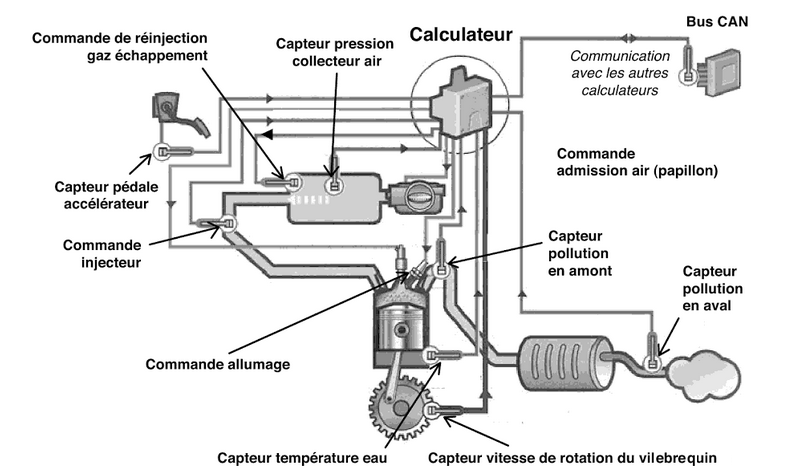
\includegraphics[height=3cm]{ControleCommande}
\end{block}

\begin{block}{Caractéristiques}

Nombreux calculateurs dédiés à des fonctions diverses : freinage ABS, gestion moteur, éclairage,
climatisation, etc.

Chaque calculateur doit optimiser un grand nombre de paramètre. Moteur à combution : pression air,
température, mélange, allumage, etc.

Le tout en temps réel et chaque calculateur est inter-dépendant avec les autres. 
\end{block}

\end{frame}

\begin{frame}[fragile]{Motivation : Contrôle--commande (suite)}

\begin{block}{Controle commande centrale nucléaire}
\begin{itemize}
 \item algorithmes contraints en temps réel
 \item Nombreux paramètres et calculs complexes
 \item Un seul c{\oe}ur de calcul peut ne pas suffir à répondre à la contrainte temps réel
 \item Exploitation de l'architecture multi-coeur : exécution concurrente de tâches \textbf{indépendantes}
\end{itemize}
\end{block}

\begin{block}{Exemple logiciel distribué : \textbf{labview}}

Le passage à la parallélisation de tâche a permis un traitement des données quinze fois plus rapide 
pour \textbf{labview} sur certaines plateformes. 

\end{block}

\end{frame}

\begin{frame}[fragile]{Motivation : Simulation de phénomènes physiques}

\begin{block}{Problème aéro--acoustique}
\center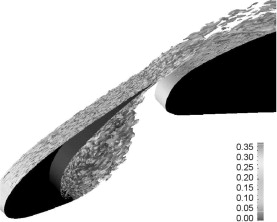
\includegraphics[height=2.5cm]{SlatWingTurb1}
\end{block}

\begin{block}{But}
calculer le bruit généré par de petites turbulences au niveau du bec de sécurité d'une aile d'avion

\begin{itemize}
\item  Petites turbulences $\Rightarrow$ modèle précis \& maillage très fin;
\item \textcolor{orange}{Sept milliards de sommets} avec 5 inconnues par sommets
\item Mémoire nécessaire : \textcolor{orange}{7 To}
\item En séquentiel : \textcolor{orange}{23 jours} pour simuler $\frac{1}{100}^{e}$ de secondes
\end{itemize}
\end{block}
\end{frame}

\begin{frame}[fragile]{Motivation : Deep Learning}

\textbf{Deep Learning} : apprentissage de modèles de données, Modélise un réseau neuronal.

\begin{itemize}
 \item internet ( reconnaissance d'images, traduction automatique, etc.)
 \item médecine ( détection cellules cancéreuses, drogues, etc.),
 \item sécurité et la défense ( détection faciale, surveillance vidéo,etc.)
 \item autonomie des machines (détection pédestre, panneaux de signalisation )
\end{itemize}

Temps d'apprentissage :
\begin{itemize}
\item Ordinateur séquentiel, apprentissage  > 1 an
\item GPGPU, en parallèle, apprentissage $\approx$ 1 mois.
\end{itemize}

Mars 2016, Alphago bat champion du monde de GO (apprentissage supervisé). \\
Octobre 2017, Alphago zero bat Alphago 100 parties à zéro (deep learning)

\end{frame}

\begin{frame}[fragile]{Motivation : Traitement de l'image}

capteurs optiques pour navigation véhicules autonomes, super résolution
sur images vidéos, etc.

\center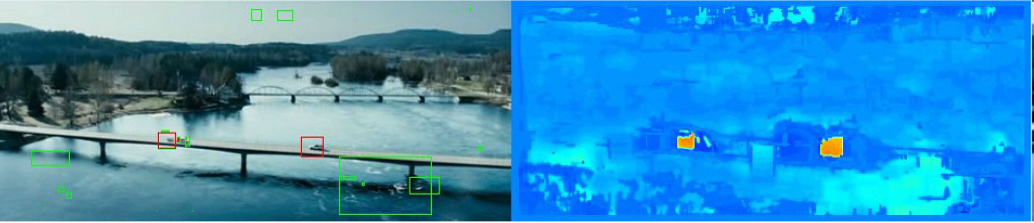
\includegraphics[height=2.5cm]{fluxvideo}

GPGPU et parallélisme permettent un traitement d'un flux vidéo à trente images par secondes
pour une résolution de $1920\times 1080$ pixels en temps réel.

\end{frame}

\section{Architecture des ordinateurs parallèles}

\begin{frame}[fragile]{Taxonomie de Flynn}
 
\begin{block}{Taxonomie de Flynn}
 
Classification faite par Michael Flynn en 1967
\small
\begin{itemize}
\item \textbf{SISD} : Simple Instruction, Simple Data : architecture classique, programmation séquentielle
  classique
\item \textbf{SIMD} : Simple Instruction, Multiple Data : Une seule instruction exécutée à la fois mais
	        appliquée sur plusieurs données simultanément : GPGPU, unités  AVX et SSE.
\item \textbf{MISD} : Multiple Instruction, Simple Data : plusieurs instructions exécutées traitant simultanément
                une seule donnée : architectures pipelines associées aux registres vectoriels.
\item \textbf{MIMD} : Multiple Instruction, Multiple Data : plusieurs instructions qui traitent chacune des données
  différentes : ordinateurs multi-c{\oe}urs, calculateurs à mémoires distribuées.
\end{itemize}
\end{block}

De nos jours, un ordinateur possède plusieurs architectures parallèles.

\end{frame}

\subsection{Architecture SIMD}

\begin{frame}[fragile]{Architecture SIMD}

\begin{center}
\begin{tikzpicture}
\node[fill=cyan, draw, rotate=90] (Data) {Données};
\node[right=10ex of Data.south ] (UC0) {\phantom{\LARGE UC}};
\node[fill= orange, circle,draw,left=2em of UC0.north, inner sep=1pt] (UC1) {\scriptsize UC};
\node[fill= orange, circle,draw,right=2em of UC0.north, inner sep=1pt] (UC2) {\scriptsize UC};
\node[fill= orange, circle,draw,left=2em of UC0.south, inner sep=1pt] (UC3) {\scriptsize UC};
\node[fill= orange, circle,draw,right=2em of UC0.south, inner sep=1pt] (UC4) {\scriptsize UC};
\node[fill=yellow, draw, above=10ex of UC0.north] (I) {Instructions};
\draw[-latex,red] (Data.340) -- (UC2.135);
\draw[-latex,red] (Data.300) -- (UC1);
\draw[-latex,red] (Data.200) -- (UC4.225);
\draw[-latex,red] (Data.240) -- (UC3);
\draw[blue] (I) -- (UC0.center);
\draw[-latex, blue] (UC0.center) -- (UC1.east);
\draw[-latex, blue] (UC0.center) -- (UC3.east);
\draw[-latex, blue] (UC0.center) -- (UC2.west);
\draw[-latex, blue] (UC0.center) -- (UC4.west);
\end{tikzpicture}
\end{center}

Une unique instruction est exécutée simultanément par tous les unités de calcul
sur ce type de machine, sur des données différentes.

\end{frame}

\begin{frame}[fragile]{Architecture SIMD (suite)}

\begin{itemize}
\item Mise en {\oe}uvre des algorithmes délicat.
\item Instructions demandant sauts conditionnels très pénalisantes
\item On utilise une technique de masque pour les sauts conditionnels.
\end{itemize}

\underline{Pour traiter les branches conditionnelles} :

\begin{minipage}[t]{0.22\textwidth}
\underline{\textcolor{blue}{Code d'origine}}

 \begin{lstlisting}[language=C++]
if ( a[i]>= 0 )
  b[i] = c[i];
else
  b[i] = -d[i];
\end{lstlisting}
\end{minipage}
\hspace{1mm}
\begin{minipage}[t]{0.65\textwidth}
\underline{\textcolor{orange}{Code compilé pour la machine}}
\begin{lstlisting}[language=C++]
msk[i] = (a[i]>=0);// = 1 si vrai, 0 sinon
b[i] = msk[i] * c[i] - (1-msk[i]) * d[i];
\end{lstlisting}
\end{minipage}
\end{frame}

\begin{frame}[fragile]{Les boucles conditionnelles en SIMD}

\underline{\textcolor{blue}{Exemple}} : boucle sur suites de Mandelbrot 
\begin{itemize}
 \item On calcule $N$ suites $z[i]$ avec $z_{n+1}[i] = z^{2}_{n}[i] + c[i]$ avec $c[i]$ complexe de module inférieur à deux.
 \item Pour chaque suite, converge ? diverge ?
 \item Diverge si $\left|z_{n}[i]\right| \geq 2$. On arrête de calculer la suite
 \item Arrêt au bout de \texttt{nIterMax} 

\end{itemize}

\begin{block}{Code classique pour calculer la $i^{e}$ suite de Mandelbrot}

\begin{lstlisting}[language=C++]
const long nIterMax = 65000;
z[i] = 0;
iter[i] = 0;
while ( (abs (z[i] ) < 2) && (iter[i] < nIterMax) )
{
  z[i] = z[i]*z[i]+c[i];
  iter[i] += 1;
}
\end{lstlisting}
\end{block}
\end{frame}

\begin{frame}[fragile]{Les boucles conditionnelles en SIMD (suite)}

\begin{itemize}
\item Chaque unité de calcul doit itérer tant qu'une des suites n'a pas divergé;
\item Utilisation système de masque pour que suites divergentes stagnent;
\item On suppose unité dotée d'une instruction de réduction permettant de savoir si un des
masques est vrai : \lstinline@reduce(msk, op::or)@ effectue un ou logique sur toutes les
valeurs de msk.
\end{itemize}

\begin{alertblock}{Code transformé}

\begin{lstlisting}[language=C++]
const long nIterMax = 65000;
z[i] = 0;
iter[i] = 0;
msk[i] = true;
while reduce(msk, op::or) 
{// Tant qu'un des masques d'une UC est vrai
  z[i] = msk[i]*(z[i]*z[i]+c[i]) + (1-msk[i])*z[i];
  iter[i] += msk[i];
  msk[i] = (abs (z[i]) < 2) && (iter[i] < nIterMax);
}
\end{lstlisting}
\end{alertblock}
\end{frame}

\begin{frame}[fragile]{Bilan des sauts conditionnels sur SIMD}
 
 \begin{block}{En résumé}
 \begin{itemize}
  \item Les sauts conditionnels en SIMD sont traduits à l'aide d'une gestion de masque;
  \item Cependant cela à un coût important puisqu'une unité de calcul SIMD doit toujours exécuter
        les deux branchements et non l'un ou l'autre;
   \item La longueur des instructions dans chaque branche doit être limitée.
   \item Il faut donc éviter au possible les sauts conditionnels !
 \end{itemize}
 \end{block}

\end{frame}

\subsection{Architecture MISD}

\begin{frame}[fragile]{Architecture MISD}

\begin{center}
\begin{tikzpicture}
\node[fill=cyan, draw, rotate=90] (Data) {Données};
\node[right=10ex of Data.south ] (UC0) {\phantom{\LARGE UC}};
\node[fill= orange, circle,draw,left=2em of UC0.north, inner sep=1pt] (UC1) {\scriptsize UC};
\node[fill= orange, circle,draw,right=2em of UC0.north, inner sep=1pt] (UC2) {\scriptsize UC};
\node[fill= orange, circle,draw,left=2em of UC0.south, inner sep=1pt] (UC3) {\scriptsize UC};
\node[fill= orange, circle,draw,right=2em of UC0.south, inner sep=1pt] (UC4) {\scriptsize UC};
\node[fill=yellow, draw, above=10ex of UC0.north] (I) {Instructions};
\draw[-latex,blue] (I.340) to[bend left] (UC4.45);
\draw[-latex,blue] (I.300) -- (UC2);
\draw[-latex,blue] (I.200) to[bend right] (UC3.135);
\draw[-latex,blue] (I.240) -- (UC1);
\draw[red] (Data) -- (UC0.center);
\draw[-latex, red] (UC0.center) -- (UC1.east);
\draw[-latex, red] (UC0.center) -- (UC3.east);
\draw[-latex, red] (UC0.center) -- (UC2.west);
\draw[-latex, red] (UC0.center) -- (UC4.west);
\end{tikzpicture}
\end{center}

Plusieurs unités de calcul vont effectuer des opérations sur le même registre ( en principe, un registre vectoriel ),
mais sur des parties différentes du registre.

\end{frame}

\begin{frame}[fragile]{Architecture MISD (suite)}

Ce type d'architecture recouvre actuellement les architectures pipelines associées 
à des registres vectoriels ( SSE -- AVX ) sur les processeurs modernes :

\begin{lstlisting}[language=C++]
for ( int i = 1; i <= 4; ++i )
  r[i] = a[i] + b[i];
\end{lstlisting}

{\scriptsize
\begin{tikzpicture}
\matrix (timeline) [matrix of nodes,nodes={draw,text width=12	mm}]
{
  Lire $a_{1}$ & Lire $a_{2}$ & Lire $a_{3}$ & Lire $a_{4}$ &              &              & \\
               & Lire $b_{1}$ & Lire $b_{2}$ & Lire $b_{3}$ & Lire $b_{4}$ &              & \\
               &              &$a_{1}+b_{1}$ &$a_{2}+b_{2}$ &$a_{3}+b_{3}$ &$a_{4}+b_{4}$ & \\
| [draw=none] | \phantom{a} & & & Écrire $r_{1}$ &Écrire $r_{2}$&Écrire $r_{3}$&Écrire $r_{4}$ \\
};
\node[below left=1em of timeline-4-1.south west]  (a00) {};
\node[below right=1em of timeline-4-7.south east] (a01) {};
\node[above left=1em of timeline-1-1.north west]  (a10) {};
\draw[thick,red,->,>=latex] (a00) to node[below]{Temps} (a01);
\draw[thick,blue,->,>=latex] (a00) to node[above,sloped]{Instructions} (a10);
\end{tikzpicture}
}

On remplit les registres vectoriels en même temps qu'on commence l'addition sur les parties des registres
de $a$ et $b$ déjà remplies.

\end{frame}

\subsection{Architecture MIMD}

\begin{frame}[fragile]{Architecture MIMD}

\begin{center}
 \begin{tikzpicture}
\node[fill=cyan, draw, rotate=90] (Data) {Données};
\node[right=10ex of Data.south ] (UC0) {\phantom{\LARGE UC}};
\node[fill= orange, circle,draw,left=2em of UC0.north, inner sep=1pt] (UC1) {\scriptsize UC};
\node[fill= orange, circle,draw,right=2em of UC0.north, inner sep=1pt] (UC2) {\scriptsize UC};
\node[fill= orange, circle,draw,left=2em of UC0.south, inner sep=1pt] (UC3) {\scriptsize UC};
\node[fill= orange, circle,draw,right=2em of UC0.south, inner sep=1pt] (UC4) {\scriptsize UC};
\node[fill=yellow, draw, above=10ex of UC0.north] (I) {Instructions};
\draw[-latex,blue] (I.340) to[bend left] (UC4.45);
\draw[-latex,blue] (I.300) -- (UC2);
\draw[-latex,blue] (I.200) to[bend right] (UC3.135);
\draw[-latex,blue] (I.240) -- (UC1);
\draw[-latex,red] (Data.340) -- (UC2.135);
\draw[-latex,red] (Data.300) -- (UC1);
\draw[-latex,red] (Data.200) -- (UC4.225);
\draw[-latex,red] (Data.240) -- (UC3);
\end{tikzpicture}
\end{center}

Cette architecture couvre une large gamme de machines, et est la plus commune actuellement :

\begin{itemize}
 \item Les PCs actuels avec leurs multi-c{\oe}urs;
 \item Les calculateurs à mémoire distribuée ou NUMA;
 \item LES GPGPUs et leurs différentes unités de calculs.
\end{itemize}

\end{frame}

\section{Mémoire partagée, mémoire distribuée et mémoire NUMA}

\begin{frame}[fragile]{Performance relative de la mémoire vive}
 Composant de l'ordinateur limitant actuellement la vitesse de traitement des données :
 
\begin{center}
{\scriptsize
\begin{tikzpicture}[scale=0.6]
\draw[->,>=latex] (0,0) -- (10,0);
\draw[->,>=latex] (0,0) -- (0,10);
\foreach \x/\xtext in {0/1980,2/1985, 4/1990, 6/1995, 8/2000, 10/2005} {
  \draw (\x,0) -- (\x,-1mm) node[below]{\xtext};
}
\foreach \y/\ytext in {0/1, 2/10, 4/100, 6/10^3, 8/10^4, 10/10^5} {
  \draw[dashed,ocre] (-1mm, \y) node[black,left]{$\ytext$} -- (10, \y);
}
\draw[blue] (0,0) -- (2.5,1.6) -- node[above,black]{CPU} (10,8.25);
\draw[red] (0,0) -- node[black,above]{Mémoire} (10,1.8);
\node[black] at (5,9) {Performances relatives à celles de 1980};
\end{tikzpicture}
}
\end{center}

\end{frame}

\subsection{Mémoire partagée}

\begin{frame}[fragile]{La mémoire partagée}
 Les unités de calcul partagent la même mémoire centrale au travers d'un bus mémoire.

 La vitesse d'accès à la mémoire vive devenue critique pour les codes actuels.
 
 Comment accélérer l'accès aux données ?
 
 Principalement deux techniques complémentaires :
 \begin{itemize}
  \item La mémoire vive entrelacée;
  \item Une mémoire cache hiérarchique;
 \end{itemize}
\end{frame}

\subsubsection{Mémoire entrelacée}

\begin{frame}[fragile]{La mémoire vive entrelacée}

\begin{itemize}
 \item Nombre de voies : Nombre de mémoire qui sont entrelacées;
 \item Largeur des voies : Nombre d'octets entre deux voies successives;
\end{itemize}

\begin{center}
 Exemple d'une mémoire entrelacée à quatre voies de largeur 3.
 
 \begin{tikzpicture}[scale=0.25]
  \foreach \x/\col in {1/red,2/violet,3/ocre,4/blue,5/red,6/violet,7/ocre,8/blue,9/red}{
    \draw[fill=\col] (3*\x,0) rectangle ++(3,1);
    \draw (3*\x,0) -- (3*\x,1);
    \draw (3*\x+1,0) -- (3*\x+1,1);
    \draw (3*\x+2,0) -- (3*\x+2,1);
  }
 \end{tikzpicture}
 
 Un carré = un octet
\end{center}

Le bloc $i, i\in \left[0, n-1\right]$ contient toutes les cellules dont les adresses sont égales à 
  $w\times ( n \times a + i ) +  k $ avec $k\in \left[0,w-1\right]$ et $a\in \mathds{N}$. 

\end{frame}

\begin{frame}[fragile]{La mémoire vive entrelacée (suite)}

\begin{block}{Accès à une mémoire non entrelacée}
{\scriptsize
\begin{center}
\begin{tikzpicture}[scale=0.75]
\draw[->,>=latex] (0,0) -- (10,0) node[below]{cycle};
\foreach \x in {0,1,...,9} {
  \draw (\x,1mm) -- (\x,-1mm) node[below] {$\x\strut$};
}
\draw[->,>=latex,blue] (0,1.5cm) node[above,black] {Requêtes} -- (0,2mm);
\draw[->,>=latex,red] (4,1.5cm) -- (4,2mm);
\draw[->,>=latex,violet] (8,1.5cm) -- (8,2mm);

\draw[->,>=latex,blue] (4,-4ex) -- (4,-1.5cm) node[below,black]{Données};
\draw[->,>=latex,red] (8,-4ex) -- (8,-1.5cm);
\end{tikzpicture}
\end{center}
}
\end{block}

\begin{block}{Accès à une mémoire entrelacée à quatre voies}
{\scriptsize
\begin{center}
\begin{tikzpicture}[scale=0.75]
\draw[->,>=latex] (0,0) -- (10,0) node[below]{cycle};
\foreach \x in {0,1,...,9} {
  \draw (\x,1mm) -- (\x,-1mm) node[below] {$\x\strut$};
}
\draw[->,>=latex,blue] (0,1.5cm) node[above,black] {Requêtes} -- (0,2mm);
\foreach \x/\col in {1/red,2/violet,3/ocre,4/blue,5/red,6/violet,7/ocre,8/blue,9/red}{
  \draw[->,>=latex,\col] (\x,1.5cm) -- (\x,2mm);
}
\draw[->,>=latex,blue] (4,-4ex) -- (4,-1.5cm) node[below,black] {Données};
\foreach \x/\col in {5/red,6/violet,7/ocre,8/blue,9/red}{
  \draw[->,>=latex,\col] (\x,-4ex) -- (\x,-1.5cm);
}
\end{tikzpicture}
\end{center}
}
\end{block}
\end{frame}

\subsubsection{Mémoire cache}

\begin{frame}[fragile]{Organisation de la mémoire cache sur une machine multi-processeurs}
 
\begin{center}
\begin{tikzpicture}
\node[rounded corners, drop shadow,draw,fill=blue!50!white,text height=1.5ex] (M) {Mémoire vive};
\node[rounded corners, drop shadow,draw,fill=green!50!white, right= 6em of M.east, text height=1.5ex] (E) {Entrée - Sortie};
\node[below=4ex of M.south] (B) {};
\node[below=4ex of E.south] (Be) {};
\node[below=4ex of M.south west] (B0) {};
\foreach \x/\n in {1/B0,2/B1,3/B2,4/B3} {
  \node[right=4em of \n.east] (B\x) {};
  \node[below=2ex of B\x.south,draw,text width=3em] (C\x) {Cache};
  \node[below=1ex of C\x.south,draw,text width=3em] (P\x) {UC};
  \draw[ocre,thick] ($(C\x.north west)+(-0.1,0.1)$) rectangle ($(P\x.south east)+(0.1,-0.1)$);
  \draw[blue] (B\x.center) -- (C\x);
}
\node[right=4ex of B4.east] (B5) {};
\draw[blue] (B0.west) -- (B5.east);
\draw[blue] (M) -- (B.center);
\draw[blue] (E) -- (Be.center);
\node[above= 1 ex of B2.north] {Bus de données};
\end{tikzpicture}
\end{center}

Cohérence des données entre mémoires caches :

{\scriptsize
\begin{itemize}
\item Une seule mémoire cache contient la donnée : donnée valide, aucune synchronisation nécessaire;
\item Donnée partagée avec d'autres caches : vérifier à chaque accès si modifiée par d'autres processeurs et alors la marquer comme invalide.
\item Valeur modifiée dans le cache et valeur en mémoire vive plus à jour : Mettre à jour la mémoire vive si d'autres processeurs veulent lire la valeur;
\item Valeur dans la mémoire cache invalide. La prochaine lecture de cette valeur déclenchera une lecture en mémoire vive. 
\end{itemize}
}

\end{frame}

\begin{frame}[fragile]{Organisation de la mémoire cache sur une machine multi-c{\oe}ur}

\small
\begin{center}
\begin{tikzpicture}
\node[rounded corners, drop shadow,draw,fill=blue!50!white,text height=1.5ex] (M) {Mémoire vive};
\node[rounded corners, drop shadow,draw,fill=green!50!white, right= 6em of M.east, text height=1.5ex] (E) {Entrée - Sortie};
\node[below=4ex of M.south] (B) {};
\node[below=4ex of E.south] (Be) {};
\node[below=4ex of M.south west] (B0) {};
\node[right=6em of B.east] (B1) {};
\node[right=14em of B1.east] (Br) {};
\node[below=7ex of B1.south,text width = 16em,fill=cyan!25,draw,text centered] (L3) {Cache L3};
\node[below=2ex of L3.south] (BL3) {};
\node[left=3em of BL3.west,draw,text width = 4em,fill=cyan!40,text centered] (L21) {\small Cache L2};
\node[right=3em of BL3.east,draw,text width = 4em,fill=cyan!40, text centered] (L22) {\small Cache L2};

\node[below=1.5em of L21.south] (BL21) {};
\node[left=0.3em of BL21.west,draw,text width = 3.5em,fill=cyan!55, text centered] (L111) {\scriptsize Cache L1};
\node[below=1ex of L111.south,draw,text width = 3.5em,fill=red!55, text centered] (U111) {\scriptsize UC};
\draw[blue,thick] ($(U111.south west)+(-0.1,-0.1)$) rectangle ($(L111.north east)+(0.1,0.1)$);
\node[right=0.3em of BL21.east,draw,text width = 3.5em,fill=cyan!55, text centered] (L112) {\scriptsize Cache L1};
\node[below=1ex of L112.south,draw,text width = 3.5em,fill=red!55, text centered] (U112) {\scriptsize UC};
\draw[blue,thick] ($(U112.south west)+(-0.1,-0.1)$) rectangle ($(L112.north east)+(0.1,0.1)$);

\node[below=1.5em of L22.south] (BL22) {};
\node[left=0.3em of BL22.west,draw,text width = 3.5em,fill=cyan!55, text centered] (L121) {\scriptsize Cache L1};
\node[below=1ex of L121.south,draw,text width = 3.5em,fill=red!55, text centered] (U121) {\scriptsize UC};
\draw[blue,thick] ($(U121.south west)+(-0.1,-0.1)$) rectangle ($(L121.north east)+(0.1,0.1)$);
\node[right=0.3em of BL22.east,draw,text width = 3.5em,fill=cyan!55, text centered] (L122) {\scriptsize Cache L1};
\node[below=1ex of L122.south,draw,text width = 3.5em,fill=red!55, text centered] (U122) {\scriptsize UC};
\draw[blue,thick] ($(U122.south west)+(-0.1,-0.1)$) rectangle ($(L122.north east)+(0.1,0.1)$);

\draw[ocre,thick] ($(U111.south west)+(-0.2,-0.2)$) rectangle ($(L21.north -| L112.east)+(0.2,0.1)$);
\draw[ocre,thick] ($(U121.south west)+(-0.2,-0.2)$) rectangle ($(L22.north -| L122.east)+(0.2,0.1)$);

\draw[ocre!50!blue,thick] ($(U111.south west)+(-0.3,-0.3)$) rectangle ($(L3.north -| L122.east)+(0.3,0.1)$);

\draw[blue] (B0.west) -- (Br.east);
\draw[blue] (M) -- (B.center);
\draw[blue] (E) -- (Be.center);
\draw[blue] (B1.center) -- (L3);
\draw[blue!75] (L3) -- (BL3.center);
\draw[blue!75] (BL3.center) -- (L21);
\draw[blue!75] (BL3.center) -- (L22);
\draw[blue!50] (L21) -- (BL21.center);
\draw[blue!50] (BL21.center) -- (L111);
\draw[blue!50] (BL21.center) -- (L112);

\draw[blue!50] (L22) -- (BL22.center);
\draw[blue!50] (BL22.center) -- (L121);
\draw[blue!50] (BL22.center) -- (L122);
\draw[orange,dashed] (L21.south east) -- node[below] {\scriptsize \textcolor{black}{Bus}} (L22.south west);
\end{tikzpicture}
\end{center}

Même problème de cohérence des caches, mais également entre les niveaux de cache ! Complexité croissante avec le nombre de
niveau hiérarchique de cache !

\end{frame}

\subsection{Mémoire distribuée}

\begin{frame}[fragile]{Principe de la mémoire distribuée}

\begin{center}
{\scriptsize
\begin{tikzpicture}[scale=0.5]
\node[draw,fill=blue!50!white, drop shadow, rounded corners] (Ram1) {Mémoire vive};
\node[below=2ex of Ram1.south] (B1) {};
\node[left=1em of B1.west,draw,fill=red!55] (U1) {UC};
\node[right=1em of B1.east,draw,fill=red!55] (U2) {UC};
\draw[blue] (Ram1) -- (B1.center);
\draw[blue] (B1.center) -- (U1);
\draw[blue] (B1.center) -- (U2);

\node[draw,fill=blue!50!white, drop shadow, rounded corners,left=10em of Ram1.east] (Ram2) {Mémoire vive};
\node[below=2ex of Ram2.south] (B2) {};
\node[left=1em of B2.west,draw,fill=red!55] (U3) {UC};
\node[right=1em of B2.east,draw,fill=red!55] (U4) {UC};
\draw[blue] (Ram2) -- (B2.center);
\draw[blue] (B2.center) -- (U3);
\draw[blue] (B2.center) -- (U4);

\node[draw,fill=blue!50!white, drop shadow, rounded corners,left=10em of Ram2.east] (Ram3) {Mémoire vive};
\node[below=2ex of Ram3.south] (B3) {};
\node[left=1em of B3.west,draw,fill=red!55] (U5) {UC};
\node[right=1em of B3.east,draw,fill=red!55] (U6) {UC};
\draw[blue] (Ram3) -- (B3.center);
\draw[blue] (B3.center) -- (U5);
\draw[blue] (B3.center) -- (U6);

\node[above=2ex of Ram1.north] (R1) {};
\node[above=2ex of Ram2.north] (R2) {};
\node[above=2ex of Ram3.north] (R3) {};
\node[right=1em of R1.east] (R0){};
\node[left=1em of R3.west] (R4) {};
\draw[thick,red] (R0.east) -- (R1.center) -- (R2.center) node[above] {Réseau}-- (R3.center) -- (R4.west);
\draw[thick,red] (Ram1) -- (R1.center);
\draw[thick,red] (Ram2) -- (R2.center);
\draw[thick,red] (Ram3) -- (R3.center);
\end{tikzpicture}
}
\end{center}

\begin{itemize}
  \item Chaque unité de calcul possède sa propre mémoire vive : l'ensemble unité de calcul + mémoire vive est appelée \textbf{n{\oe}ud de calcul};
  \item Les données sont échangées entre les n{\oe}uds de calcul au travers soit d'un bus spécialisé soit au travers un réseau intranet dédié;
  \item Sur réseau, c'est à la charge du programmeur de transiter les données d'un n{\oe}ud à l'autre;
  \item Demande une programmation et des algorithmes spécifiques pour exploiter au mieux de type de machine;
  \item Permet d'exploiter plusieurs centaines de milliers de n{\oe}uds de calcul;
  \item Cependant limité par la consommation électrique !
 \end{itemize}

\end{frame}

\subsection{Architecture NUMA}

\begin{frame}[fragile]{Architecture NUMA}
 
\begin{center}
\begin{tikzpicture}
\node[draw,rounded corners, drop shadow, fill=ocre] (N11) {$N_{11}$};
\node[right = 2em of N11.north east,rotate=90,anchor=east, draw, fill=cyan] (M1) {Mémoire vive};
\node[left  = 2.5em of M1.north west, anchor=south, draw, fill=ocre, drop shadow, rounded corners] (N12) {$N_{12}$};
\node[right = 2em of M1.south, rounded corners, rotate = 90,drop shadow, fill=green, draw, anchor = north] (C) {Cross bar};
\node[right = 2em of C.south,rotate=90,anchor=north, draw, fill=cyan] (M2) {Mémoire vive};
\node[right  = 2.5em of M2.south east, anchor=north, draw, fill=ocre, drop shadow, rounded corners] (N21) {$N_{21}$};
\node[right  = 2.5em of M2.south west, anchor=south, draw, fill=ocre, drop shadow, rounded corners] (N22) {$N_{22}$};
\draw (N11) -- (M1);
\draw (N12) -- (M1);
\draw (N21) -- (M2);
\draw (N22) -- (M2);
\draw[dashed, thick ,red] (M1.330) -- (C);
\draw[dashed, thick ,red] (M1.210) -- (C);
\draw[dashed, thick ,red] (M2.150) -- (C);
\draw[dashed, thick ,red] (M2.30) -- (C);
\end{tikzpicture}
\end{center}

 \begin{itemize}
  \item Machine contenant des n{\oe}uds de calcul;
  \item Chaque n{\oe}ud contient plusieurs unités de calcul;
  \item Les n{\oe}uds de calcul sont reliés par un crossbar;
  \item Du point de vue programmeur, la mémoire est partagée;
  \item Mais les temps d'accès aux données varient fortement selon qu'une unité de calcul
  accède à une donnée se trouvant sur son n{\oe}ud de calcul ou sur un n{\oe}ud de calcul
  distant.
 \end{itemize}

\end{frame}

\begin{frame}[fragile]{Architecture NUMA}

\small
 \begin{itemize}
  \item On trouve des architectures NUMA dans les Xeons des processeurs INTEL. Chaque chipset est un n{\oe}	ud de calcul
  relié par un crossbar appelé \textbf{QPI} ( Quick Path Interconnect ) dans la terminologie d'INTEL;
  \item Programme classique multi-thread fonctionne mais peu optimiser;
  \item L'optimisation demande de fixer chaque thread à une unité de calcul : c'est \textbf{l'affinité};
  \item Le programmeur peut ensuite contrôler la répartition des données sur les n{\oe}uds de calcul à
  l'aide d'une politique choisie parmi les suivantes ( non exhaustive ) :
  {\scriptsize
    \begin{description}
     \item \textcolor{blue}{\textbf{defaut}} \textcolor{blue}{Allocation sur le n{\oe}ud local où s'exécute le processus}
     \item \textcolor{DarkGreen}{\textbf{First Touch Policy}} \textcolor{DarkGreen}{L'allocation ne se fait pour une page mémoire que lors du premier
     accès à une donnée de cette page. L'allocation se fait alors  pour cette page sur le n{\oe}ud local où s'exécute le processus}
     \item \textcolor{BrickRed}{\textbf{Interleaving}} \textcolor{BrickRed}{L'allocation d'un tableau se fait en distribuant de façon cyclique les pages
     mémoires sur les différents n{\oe}uds de calcul}
    \end{description}
}
 \end{itemize}
\end{frame}


\end{document}
